
\chapter{The key ideas}

% Not too long, so that it can be read quickly

\section{Introduction -- what is this book about}
Somebody who opens this book might wonder -- it this book for me? What is this book about and will I benefit from reading it?
 Many of you might have heard about INLA and have picked this book up because it has INLA in the title-- and can teach you ``How to use INLA'' or what models can be fitted with. Others might have come across this book they are familiar with INLA, but would like to see a wide  range of models that may be fitted with INLA. The things is-- this book is not about INLA.
 
In this first chapter we illustrate what this book  is about, by showing examples of a number of data structures that may be seen a typical special cases that the analysis methods discussed in this book can deal with. When reading this you may find that some of the data sets initially seem to be very different in structure. In this chapter we show the diversity and pointing out similarity.

INLA is a model fitting method -- we will discuss it in detail below -- and as such a means to an end. 
Spatial component that has not been traditionally pointed out/discussed.


\section{Examples -- data structures}

Lets have a look at a few examples of data structures.

\subsection{Spatially continuous data}
% to do:
% find appropriate data set

Consider Figure \ref{fig:elev} which shows the elevation in a rainforest study plot in Panama. In this data structure that  takes on values everywhere in the plot; there is not a single location where it would not make sense to consider elevation as the quantity is spatially continuous.
\begin{figure}
\centering
%\includegraphics[width=0.3\textwidth]{complete}
%\includegraphics[width=0.6\textwidth]{sealsscotland}
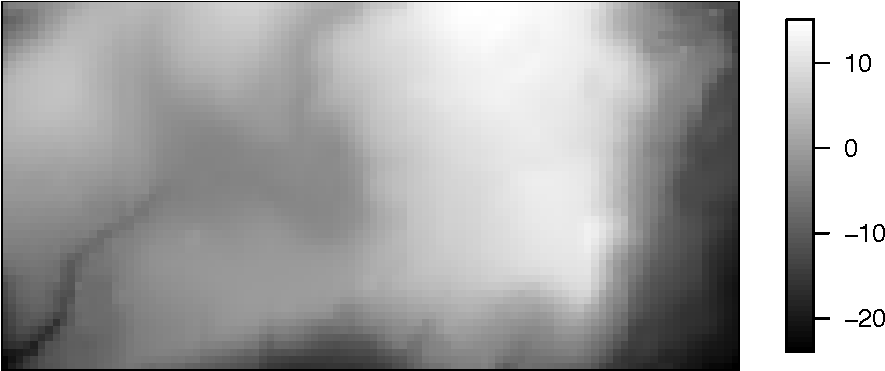
\includegraphics[width=0.6\textwidth]{elev}
\caption{\label{fig:elev} Some elevation somewhere...}
\end{figure}
In practice, however, there are limitations. While there are there are infinitely many locations in even a small area of space the quantity of interest cannot be measured everywhere in space -- and the quantity of interest cannot be fully observed. It can only be measured at a finite number of locations and these location have typically been chosen as part of the study design. There is an interest in interpolating to locations where no measurements have been taken -- referred to as \textit{spatial prediction}. This prediction into other areas of space needs to be done in a clever way, that take into account information from given measurements. In particular, on would like the predicted values to be similar to the values measured in the other locations. The figure is actually based on XX measurements in as many locations randomly distributed across the plot. There might also be an interest in relate one spatially continuous variable to other spatially continuous variables as part of a modelling exercise. These spatial covariates might help to explaining why values are high/low in different areas of the plot, but there might still be spatial structure left that needs to be accounted for.

This data structure is often referred to as \textit{geo-referenced data}\index{geo-referenced data} or \textit{geostatistical data}\index{geostatistical data}.

\subsection{Spatial point patterns}
Figure \ref{fig:rainpattern} shows  the same rainforest study plot as Figure \ref{fig:elev}, but this time the locations of trees of the species \textit{Beilschmidia} have been plotted. A study might be interested in analysing the pattern formed by those trees to understand habitat preferences of the species. Hence, unlike in the previous example the locations have not been deliberately chosen as part of the study but are the object of interest. The main interest is to understand-- and hence model the spatial pattern.
Again, spatial covariates might explain the spatial pattern but there might still be spatial structure left that needs to be accounted for.

This data structure is referred to as a \textit{spatial point pattern}\index{spatial point pattern}.
\begin{figure}
\centering
%\includegraphics[width=0.3\textwidth]{complete}
%\includegraphics[width=0.6\textwidth]{sealsscotland}
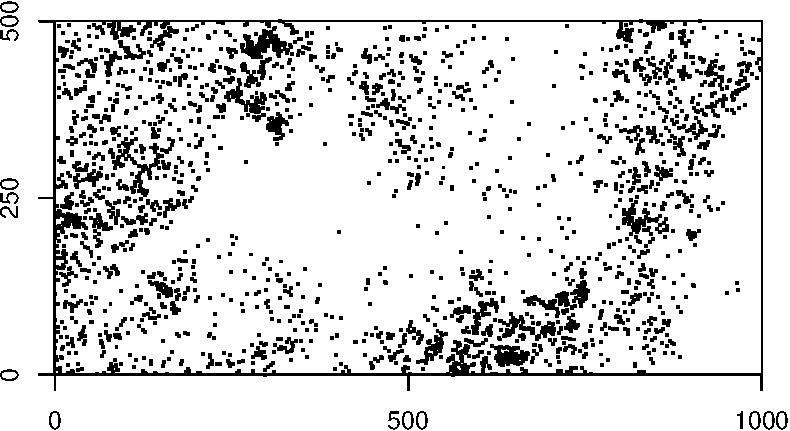
\includegraphics[width=0.6\textwidth]{rain_pattern}
\caption{\label{fig:rainpattern} Rainforest trees...}
\end{figure}




\subsection{Data collected on transects}
\subsection{Distance sampling data}


\section{Synergy -- common spatial structure}
Datasets collected in different ways -- but the all have 
a spatial structure. Spatial structure is relevant, of interest or might impact on inference.

How do we represent this spatial structure? This is how 

\subsection{The random field -- intuition}



\subsection{Issues with spatial data analysis}

Computationally complex. Hence need to be computationally efficient.

Need to approximate.

Space is complex (sphere, holes) -- need to be flexible. Grids are rigid... 

\section{What to expect from the book}


Finding a rigorous yet flexible way of representing the spatial structure and linking this with computationally efficient model fitting strategies that allow us to fit relevant and realistically complex models.

\section{Structure of the book}

Next Chapter explores key concepts by referring to the different data structures we have seen here. It ends with a roadmap of this book.
 
Chapter after that formalises these concepts



